
\section{The Volatility of Peace}

\subsection{Volatility Without Violence}

\textbf{What broke it was what no one expected: a tarrif deal.}

\begin{HistoricalSidebar}{When Markets Feared Peace}

  Markets hate uncertainty. Howevdr, they hate unpriced reversals even more.

  \medskip
  
  Most market narratives focus on the shocks of war. But sometimes, it’s the \textit{absence} of war — or the sudden 
  appearance of peace — that triggers the sharpest repricings.

  \medskip
  
  In \textbf{1973}, the Yom Kippur War triggered an oil embargo by OPEC, sending crude prices quadrupling in just months. 
  Traders learned to fear geopolitical flashpoints.

  \medskip
  
  But in \textbf{1979}, a different kind of whiplash occurred.

  \medskip
  
  After years of tension and violence in Iran, the initial reaction was panic when the Shah fell: 
  production disruptions, 
  regime uncertainty, and another spike in oil. Yet within months, backchannel diplomacy hinted 
  at stabilization. Export 
  routes reopened. Fears of an extended conflict began to fade.

  \medskip
  
  Then came the surprise: oil futures collapsed.

  \medskip
  
  Not because of war — but because it didn’t continue.

  \medskip
  
  Funds that had positioned themselves for prolonged geopolitical strife were caught leaning the wrong way. Inventories 
  overshot. Tankers rerouted. And speculative longs that were built on the expectation of chaos started to unwind 
  violently.
  
  \medskip
  
  \textbf{The lesson?} Peace is only stabilizing if it’s priced in.

  \medskip
  
  Otherwise, it behaves just like a crisis.
  
\end{HistoricalSidebar}

For weeks, global markets had been pricing in a tariff war. 

It was like a casino full of traders who'd all heard the same rumor about rising barriers.  

The rumor? That negotiations had collapsed for good: retaliatory duties incoming, supply chains fracturing, and container 
ships rerouted overnight.


The bet was simple: if supply gets choked then prices go up.

\medskip

\begin{figure}[H]
  \centering
  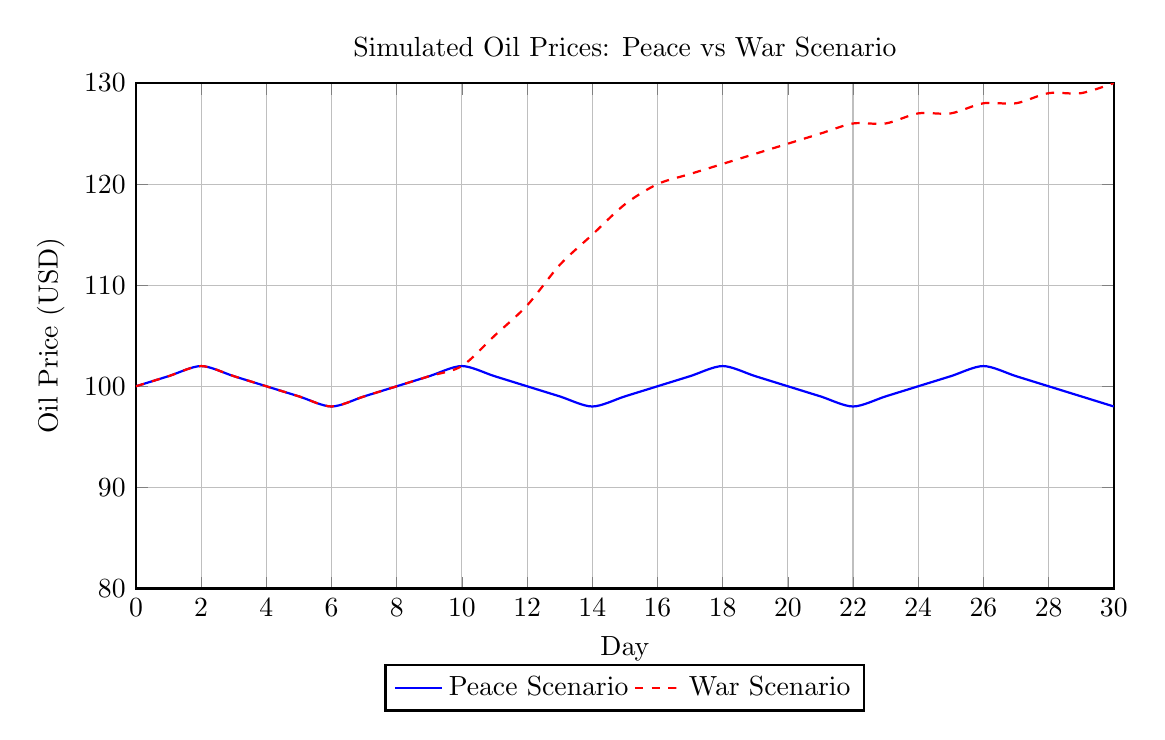
\begin{tikzpicture}
    \begin{axis}[
      width=14cm,
      height=8cm,
      xlabel={Day},
      ylabel={Oil Price (USD)},
      title={Simulated Oil Prices: Peace vs War Scenario},
      legend style={at={(0.5,-0.15)}, anchor=north, legend columns=2},
      grid=both,
      ymin=80, ymax=130,
      xmin=0, xmax=30,
      thick
    ]
  
    % Peace Scenario
    \addplot[
      color=blue,
      mark=none,
      smooth
    ] table[row sep=\\] {
      x y \\
      0 100 \\
      1 101 \\
      2 102 \\
      3 101 \\
      4 100 \\
      5 99 \\
      6 98 \\
      7 99 \\
      8 100 \\
      9 101 \\
      10 102 \\
      11 101 \\
      12 100 \\
      13 99 \\
      14 98 \\
      15 99 \\
      16 100 \\
      17 101 \\
      18 102 \\
      19 101 \\
      20 100 \\
      21 99 \\
      22 98 \\
      23 99 \\
      24 100 \\
      25 101 \\
      26 102 \\
      27 101 \\
      28 100 \\
      29 99 \\
      30 98 \\
    };
    \addlegendentry{Peace Scenario}
  
    % War Scenario
    \addplot[
      color=red,
      mark=none,
      dashed,
      smooth
    ] table[row sep=\\] {
      x y \\
      0 100 \\
      1 101 \\
      2 102 \\
      3 101 \\
      4 100 \\
      5 99 \\
      6 98 \\
      7 99 \\
      8 100 \\
      9 101 \\
      10 102 \\
      11 105 \\
      12 108 \\
      13 112 \\
      14 115 \\
      15 118 \\
      16 120 \\
      17 121 \\
      18 122 \\
      19 123 \\
      20 124 \\
      21 125 \\
      22 126 \\
      23 126 \\
      24 127 \\
      25 127 \\
      26 128 \\
      27 128 \\
      28 129 \\
      29 129 \\
      30 130 \\
    };
    \addlegendentry{War Scenario}
  
    \end{axis}
  \end{tikzpicture}
  \caption{Simulated oil prices under Peace vs War conditions over 30 days.}
\end{figure}

\medskip


If oil futures surged then crude flirted with triple digits.

Investment desks positioned themselves accordingly. 
Energy portfolios were stacked with long positions. It is the financial equivalent of stockpiling 
canned food before a hurricane. 
The hedge funds placed their leveraged bets. 
The sovereign wealth funds adjusted their allocations. 
Even cautious family offices
\footnote{Family offices are investment management structures established by wealthy families to manage and 
grow their wealth, across generations.}, 
the financial turtles of the investing world, crept into the action, 
betting on the storm lasting.

But here’s the catch:
\textbf{All these trades were modeled on the assumption of gridlock.}
and that energy would become the world’s next great bottleneck.

\medskip

\begin{figure}[H]
  \centering
  \begin{tikzpicture}[scale=1.1]
  
    % Nodes for regions
    \node[draw, fill=blue!10, minimum width=2cm, minimum height=1cm, rounded corners] at (-5, 0) (Americas) {Americas};
    \node[draw, fill=green!10, minimum width=2cm, minimum height=1cm, rounded corners] at (0, 2) (Europe) {Europe};
    \node[draw, fill=yellow!10, minimum width=2cm, minimum height=1cm, rounded corners] at (4, 0) (Asia) {Asia};
    \node[draw, fill=orange!10, minimum width=2cm, minimum height=1cm, rounded corners] at (0, -2) (Mideast) {Mideast};
  
    % -- Conflict Scenario (gray dashed reroutes) --
    \draw[->, thick, dashed, gray] (Americas.east) .. controls (-2,0.5) .. (Europe.west) node[midway, above, font=\scriptsize, gray] {rerouted};
    \draw[->, thick, dashed, gray] (Europe.east) .. controls (2,1.5) .. (Asia.west);
    \draw[->, thick, dashed, gray] (Asia.south west) .. controls (2.5,-1.5) .. (Mideast.east);
  
    % -- Peace Scenario (bold reactivated routes) --
    \draw[->, thick, blue] (Americas.east) .. controls (-1,1.5) .. (Asia.west) node[midway, above, font=\scriptsize, blue!70!black] {reactivated};
    \draw[->, thick, blue] (Mideast.north) -- (Europe.south) node[midway, right, font=\scriptsize, blue!70!black] {normal flow};
  
    % Blocked zone icon (conflict assumption)
    \draw[thick, red] (0.5,-0.4) circle (0.4cm);
    \node[red, font=\scriptsize] at (0.5,-1.1) {Chokepoint};
  
    % Peace unlocked symbol
    \node[font=\Large, blue!80!black] at (0.5,-0.4) {\checkmark};
  
    % Caption
    \node[align=center, font=\small, text width=10cm, below=2.5cm of Mideast.south] {
      \textbf{Market Assumptions:} Trade routes blocked due to conflict (gray, dashed)\\
      \textbf{What Happened:} Routes reopened suddenly (blue, solid) as diplomacy unexpectedly succeeded.
    };
  
  \end{tikzpicture}
  \caption{Simplified trade flow map: models priced in conflict and rerouting, but peace reactivated critical corridors and shocked market expectations.}
\end{figure}

\medskip

In trading terms, this was a textbook ``consensus narrative'': a shared story that underwrites the price of everything 
from oil futures to airline stocks. It’s like everyone agreeing the bridge ahead is broken and adjusting their GPS 
routes accordingly. If that bridge suddenly reopens? Chaos. Price reversion. And margin calls for anyone who bet too 
heavily on detours.

In short: the markets weren't just betting on oil.
They were betting on stalemate.
And when stalemates break, so do assumptions.

\medskip

\begin{PhilosophicalSidebar}{The Consensus Narrative}

  Markets don’t just price assets.  
  They price stories.

  \medskip
  
  A \textbf{consensus narrative} is the shared fiction everyone agrees to believe — not because it's true, but because 
  it’s \textit{useful}.  Like money. Like borders. Like market confidence itself.
  
  \medskip

  In theory, prices are objective: functions of supply, demand, and discounted cash flows.  
  In practice, they’re often anchored to collective expectations — war drags on, interest rates stay flat, demand rebounds, 
  volatility remains containable.

  \medskip
  
  When those expectations are stable, so are markets.  
  But consensus isn’t knowledge. It’s choreography.  
  Everyone adjusts their models not to reality, but to what they think others believe reality will be.
  
  \medskip
  
  This is where philosophy meets finance.  
  David Hume warned that causality itself is inferred — not seen.  
  Thomas Kuhn showed how science advances through “paradigm shifts,” not incremental truth.  
  And George Soros built a hedge fund empire on reflexivity — the idea that markets move not toward reality, but toward the 
  beliefs they manufacture and reinforce.
  
  \medskip
  
  So when traders say “the market priced in a stalemate,” they don’t mean it’s true.  
  They mean it’s operationally assumed.

  \medskip
  
  The danger?  
  Consensus narratives are stable — until they’re not.  
  When the story breaks, the model doesn’t just shift.  
  It collapses.  

  \medskip
  
  And that collapse doesn’t just create volatility.  
  It creates \textbf{epistemic whiplash} — the sudden, violent shock of realizing the map wasn’t the territory.
  
\end{PhilosophicalSidebar}

\medskip


Then came the de-escalation.

A late-night breakthrough in trade talks, capped by a surprise joint statement. Suddenly, tariff schedules were 
suspended and reciprocal duties rolled back.  
Within minutes, logistics networks recalibrated. Container bookings resumed. Supply chains that had been pricing 
in disruption began breathing again.

\textbf{And with that, oil futures dropped 14\% in 15 minutes.}

The geopolitical script flipped overnight. The expected standoff didn’t materialize because a surprise 
deal was inked. 

And just like that, the market re-priced violently.

Imagine a packed theater where the audience has been told the fire alarm is just part of the show, and then someone 
yells “actual fire.” The rush for the exits isn’t graceful. 

But that wasn’t the only surprise: Credit spreads blew out, but not where the models were looking.

\medskip

\begin{figure}[H]
  \centering
  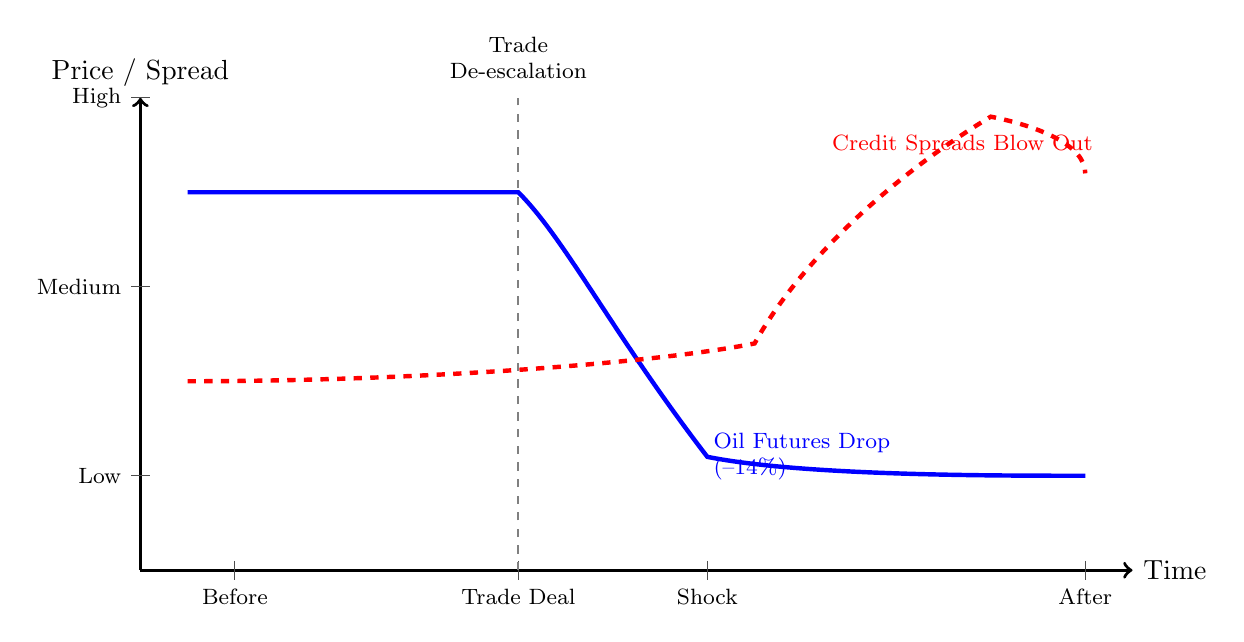
\begin{tikzpicture}[
      scale=1.2,
      axis/.style={very thick, ->},
      oil/.style={ultra thick, blue},
      credit/.style={ultra thick, red, dashed},
      tick/.style={black!70},
      label/.style={font=\footnotesize},
      note/.style={font=\footnotesize, align=left}
    ]

    % Axes
    \draw[axis] (0,0) -- (10.5,0) node[right] {Time};
    \draw[axis] (0,0) -- (0,5) node[above] {Price / Spread};

    % Time ticks
    \foreach \x/\label in {1/Before, 4/Trade Deal, 6/Shock, 10/After} {
      \draw[tick] (\x,0.1) -- (\x,-0.1);
      \node[label, below] at (\x,-0.1) {\label};
    }

    % Price ticks
    \foreach \y/\label in {1/Low, 3/Medium, 5/High} {
      \draw[tick] (0.1,\y) -- (-0.1,\y);
      \node[label, left] at (-0.1,\y) {\label};
    }

    % Oil Futures Drop (blue)
    \draw[oil] 
      (0.5,4) 
      .. controls (2,4) and (3.5,4) .. (4,4)
      .. controls (4.5,3.5) and (5,2.5) .. (6,1.2)
      .. controls (7,1) and (9,1) .. (10,1);

    % Credit Spread Spike (red dashed)
    \draw[credit]
      (0.5,2)
      .. controls (3,2) and (5.5,2.2) .. (6.5,2.4)
      .. controls (7,3.3) and (8,4.2) .. (9,4.8)
      .. controls (9.5,4.7) and (10,4.5) .. (10,4.2);

    % Labels
    \node[note, blue] at (7,1.2) {Oil Futures Drop \\ (–14\%)};
    \node[note, red] at (8.7,4.5) {Credit Spreads Blow Out};

    % Vertical annotation line for Trade Deal
    \draw[dashed, thick, gray] (4,0) -- (4,5);
    \node[label, above, align=center] at (4,5.1) {Trade\\De-escalation};

  \end{tikzpicture}
  \caption{Financial Response to Sudden Trade De-escalation: Oil Futures and Credit Spreads}
\end{figure}


\medskip


In financial terms, a “credit spread” is like an insurance premium. 
It’s how much extra return an investor demands to lend money to a risky borrower instead of a safe one. 
When spreads “blow out,” it means people suddenly see more risk and demand more compensation to take it on.
It is like an earthquake making everyone scramble to check their home insurance policy.

\medskip

\begin{TechnicalSidebar}{Credit Spreads and the Anatomy of a Blowout}
  In traditional finance, a \textbf{credit spread} measures the difference in yield between a corporate bond and a 
  risk-free government bond of comparable maturity. It reflects the market’s perception of default risk. A higher 
  spread signals higher perceived risk; a lower spread suggests confidence in repayment.
  
  \medskip
  
  \textbf{The Baseline:}  

  \medskip

  If the U.S. 10-year Treasury is yielding 2.0\% and a corporate bond yields 6.0\%, the credit spread is:
  \[
  6.0\% - 2.0\% = 4.0\%
  \]

  \medskip
  
  This 4.0\% “risk premium” compensates investors for the possibility of default.
  
  \medskip

  A \textbf{credit spread blowout} occurs when spreads widen rapidly across a category of borrowers; especially 
  high-yield or speculative-grade issuers. It often precedes or coincides with a liquidity crisis, as lenders 
  demand dramatically higher yields or refuse to roll debt entirely.
  
  \medskip
  
  \textbf{Historical Blowouts:}

  \medskip

  \begin{itemize}
    \item \textbf{2008 Financial Crisis:} Spreads on junk bonds exceeded 2,000 basis points (20\%), reflecting panic 
    over cascading defaults.
    \item \textbf{COVID-19 March 2020:} Even investment-grade spreads widened dramatically until the Fed intervened 
    with corporate bond purchases.
  \end{itemize}

  \medskip

  A spread blowout doesn’t just reflect risk. It creates it. It signals that markets are no longer willing to fund 
  at previous terms. For leveraged firms, that can trigger a debt rollover crisis, margin calls, or forced liquidation 
  — especially when \textbf{credit was being used to simulate liquidity}.

\end{TechnicalSidebar}

\medskip

But here’s the twist: The quake didn’t hit where the seismographs were pointed.

Traders had positioned themselves around the obvious fault lines: energy companies, defense contractors, and countries caught 
in the geopolitical blast radius. The models were calibrated to stress those areas. Risk was priced-in there.

But the actual rupture came somewhere else. It was like boarding up your windows for a hurricane, only to have the roof collapse 
from termites you didn’t even know were there.

When the unexpected sector starts flashing red, credit spreads widen there, liquidity dries up, and everyone who thought 
they were safe suddenly isn’t. The models were wrong because the world refused 
to stay inside the prediction box.

\medskip

\begin{figure}[H]
  \centering
  \begin{tikzpicture}
    \matrix[matrix of nodes,
            nodes={minimum height=1cm, minimum width=1.8cm, text width=1.8cm, align=center},
            column sep=0.1cm, row sep=0.1cm,
            cells={nodes={draw, font=\small}}] (m) {
      |[fill=red!70]| Energy & |[fill=orange!30]| Shipping & |[fill=green!10]| Regional Banks & |[fill=yellow!20]| Real Estate & |[fill=green!10]| Tech \\
      |[fill=orange!20]| Energy & |[fill=red!70]| Shipping & |[fill=red!60]| Regional Banks & |[fill=yellow!30]| Real Estate & |[fill=green!10]| Tech \\
    };
  
    % Labels
    \node[font=\bfseries] at ($(m-1-1.north west)!0.5!(m-1-5.north east)+(0,1)$) {Expected Credit Spread Stress};
    \node[font=\bfseries] at ($(m-2-1.south west)!0.5!(m-2-5.south east)+(0,-1)$) {Actual Credit Spread Stress};
  
    % Color legend
    \begin{scope}[shift={(7.2,-0.5)}]
      \node[align=left, font=\small] at (0,1.2) {Stress Level};
      \draw[fill=green!10] (0,0.8) rectangle ++(0.4,0.4);
      \node[anchor=west, font=\tiny] at (0.5,1.0) {Low};
  
      \draw[fill=yellow!30] (0,0.3) rectangle ++(0.4,0.4);
      \node[anchor=west, font=\tiny] at (0.5,0.5) {Moderate};
  
      \draw[fill=red!70] (0,-0.2) rectangle ++(0.4,0.4);
      \node[anchor=west, font=\tiny] at (0.5,0.0) {High};
    \end{scope}
  \end{tikzpicture}
  \caption{Heatmap of Expected vs. Actual Credit Spread Movement. Models focused on obvious sectors (e.g., Energy), but market stress materialized 
  in overlooked areas like Shipping and Regional Banks.}
\end{figure}

\medskip

Most risk engines had been trained on the usual suspects.
They were like airport security trained to spot people with ticking suitcases and shady passports. The algorithms knew how to 
flag high-yield bonds from companies drowning in debt, or cyclical sectors like manufacturing and construction that wobble 
with every interest rate shift. These models were fluent in the language of fragility — companies with weak balance sheets, 
volatile revenues, or exposure to economic booms and busts.

But this time, the pressure hit from the blind side.

Instead of the usual weak links snapping, the stress landed on investment-grade borrowers — supposedly sturdy, reputable firms 
— who happened to rely on commodity-linked income or had large footprints in markets that were suddenly back in play after 
years of sanctions. These weren’t the people with ticking suitcases. These were the ones wearing business class tags and 
tailored suits. And when turbulence hit them, no one saw it coming.

\medskip

\begin{figure}[H]
  \centering
  
  % === First row: Conflict Shock ===
  \begin{subfigure}[t]{0.45\textwidth}
  \centering
  \begin{tikzpicture}
    \comicpanel{0}{0}
      {Risk Analyst}
      {Macro Analyst}
      {Rising tension. Sanctions expected. Volatility will spike in energy and defense.}
      {(-0.6,-0.6)}
  \end{tikzpicture}
  \caption*{Conflict shock: the volatility is forecast, localized, and priced in.}
  \end{subfigure}
  \hfill
  \begin{subfigure}[t]{0.45\textwidth}
  \centering
  \begin{tikzpicture}
    \comicpanel{0}{0}
      {Risk Analyst}
      {Macro Model}
      {Contagion risk remains in the usual suspects: cyclicals, high-yield, frontier markets.}
      {(0.6,-0.6)}
  \end{tikzpicture}
  \caption*{The usual drill: stress ripples through known fault lines.}
  \end{subfigure}
  
  \vspace{1em}
  
  % === Second row: Peace Shock ===
  \begin{subfigure}[t]{0.45\textwidth}
  \centering
  \begin{tikzpicture}
    \comicpanel{0}{0}
      {Risk Analyst}
      {Macro Analyst}
      {Ceasefire? Trade lanes reopening? This wasn't in the training data.}
      {(-0.6,-0.6)}
  \end{tikzpicture}
  \caption*{Peace shock: the models aren’t built to process resolution.}
  \end{subfigure}
  \hfill
  \begin{subfigure}[t]{0.45\textwidth}
  \centering
  \begin{tikzpicture}
    \comicpanel{0}{0}
      {Risk Analyst}
      {Macro Analyst}
      {Credit spreads just blew out in investment-grade shipping. Why now?}
      {(0.6,-0.6)}
  \end{tikzpicture}
  \caption*{The misfire: volatility hits where “peace” broke the assumptions.}
  \end{subfigure}
  
  \caption*{Markets don’t just panic when things get worse. Sometimes they panic when things get better.}
\end{figure}

\medskip


The underlying math was based on the idea 
that bad news spreads quickly and good news doesn’t spread at all. It assumed that volatility comes from conflict, 
and contagion from collapse. However, this time, the trigger was a peace deal. And that 
broke the logic the models were built on.

In market terms, it was like every fire drill having trained people to flee from smoke, and then discovering 
that some doors slam shut when the alarm is turned off.  Peace, it turns out, can cause a stampede too.

Because peace doesn’t usually cause flash crashes. \textit{Until it does.}



